\documentclass[12pt,onecolumn]{article}

\usepackage{xeCJK}
\usepackage{graphicx}
\usepackage{indentfirst}
\usepackage{float}

\setCJKmainfont[AutoFakeBold=0.25]{SimSun}
\setCJKsansfont[AutoFakeBold=0.25]{SimSun}
\setCJKmonofont[AutoFakeBold=0.25]{SimSun}
\setmainfont{Times New Roman}
\setsansfont{Times New Roman}
\setmonofont{Times New Roman}
\linespread{1.25}
\setlength{\parindent}{2em}

\begin{document}
    \title{人工神经网络原理文献报告}
    \author{17363092 叶茂青}

    \maketitle

    \section{Rich feature hierarchies for accurate object detection and semantic segmentation\cite{girshick2014rich}}
    提出了R-CNN这一网络架构,在传统的CNN架构上加入Region Proposal的结构,从而完成图像目标检测的任务。R-CNN完成图像目标检测的步骤如下:

    1. 使用Region proposals在原图像中取出大约2000个区域

    2. 使用一个CNN网络将提取出来的区域变为一个固定长度的特征

    3. 使用SVM进行分类

    \begin{figure}[htb]
        \centering
        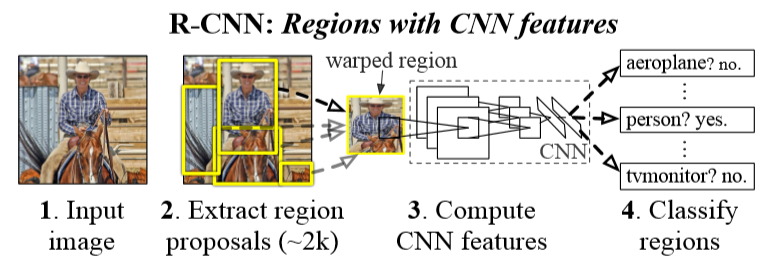
\includegraphics[width=\linewidth]{figure/rcnn.png}
        \caption{R-CNN architecture}
    \end{figure}

    第一步Region proposals的方法采用Selective search,第二步使用预训练的Alexnet对输入为$227\times 227$的RGB图片抽取4096维的特征向量,最后采用SVM进行分类,并通过回归的方法修正Bounding box的误差。

    R-CNN的一些缺点:

    1. Region proposals提取的区域会有重叠,送入CNN网络时会有很多重复计算

    2. CNN网络需要固定尺寸的图片

    3. 网络分为了多个过程,训练过程复杂

    \section{Spatial pyramid pooling in deep convolutional networks for visual recognition\cite{he2015spatial}}

    对于前面所提到的R-CNN的缺点1、2作出了一点改进,提出了一种叫做Spatial pyramid pooling network的结构。

    对于第一个缺点,通过映射关系,从featrue map中找到对应region产生的feature,从而避免重复的计算,只需要将整张图片经过一次CNN网络即可。

    对于第二个缺点,R-CNN中需要对裁剪的图像重新进行处理的原因是Alexnet最后为全连接层,需要保证输入的维数固定,Spatial pyramid pooling network通过将最后一层卷积层的输出,经过池化操作变为固定长度的特征向量,从而让网络可以接受任意大小的图片。

    \begin{figure}[htb]
        \centering
        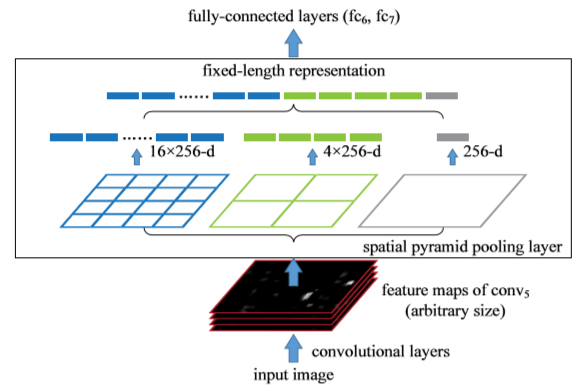
\includegraphics[width=\linewidth]{figure/spp.png}
        \caption{A network structure with a spatial pyramid pooling layer}
    \end{figure}

    如Figure 2中所示,在整幅图像的卷积结果上找到对应region产生的feature,Spatial pyramid pooling network将feature分割成16份、4份、1份,再使用Max Pooling对每一份内的特征进行池化,最后拼接起来形成$21\times dimension$的特征向量作为全连接层的输入。
    
    \section{Fast r-cnn\cite{girshick2015fast}}

    R-CNN需要把Region proposals选出的2000个区域都送入CNN进行计算,极大的降低了目标检测的效率,Fast R-CNN受Spatial pyramid pooling network的启发,在特征图上进行Region proposals。同时抛弃了R-CNN使用SVM进行分类的做法,引入multi-task loss,直接用Softmax对分类进行预测。

    Fast R-CNN的想法与Spatial pyramid pooling network中的类似,相比于Spatial pyramid pooling network中将feature做$4\times 4$、$2\times 2$、$1\times 1$的分割,Fast R-CNN提出的RoI pooling layer直接将feature划分为$7\times 7$的网格并做Max Pooling。

    其他的trick包括使用smoothL1 loss计算bounding box误差,使用SVD分解加快推测速度,采用更大的CNN网络。

    \begin{figure}[htb]
        \centering
        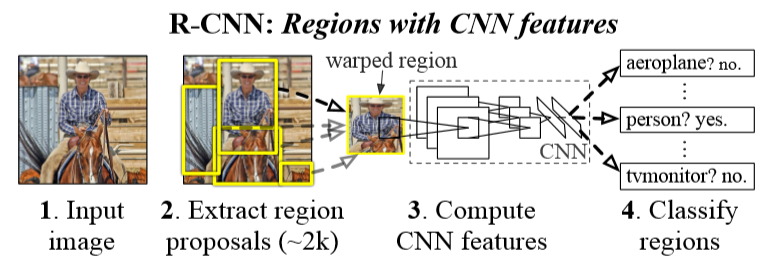
\includegraphics[width=\linewidth]{figure/rcnn.png}
        \caption{Fast R-CNN architecture}
    \end{figure}

    \section{Faster r-cnn: Towards real-time object detection with region proposal networks\cite{ren2015faster}}

    Fast R-CNN并没有完全做到end-to-end的训练,虽然只需要过一次CNN网络,但Region proposals部分依旧需要很长的时间,Faster R-CNN将Region proposals部分也融入到网络中,极大的提高了运算效率。相比之前的Selective search方法,Faster R-CNN引入了Region Proposal Networks来完成Region Proposal的任务。

    Region Proposal Networks取最后一层卷积层的输出作为输入,用sliding window(论文设定为$3\times 3$)滑过feature map,对于每一个中心点建立k个region,再交由后面的cls layer分辨是否存在物体,reg layer修正region的范围,由于实际中不包含物体的region较多,为了保证正负样本的均衡,在每副图像上随机采样256个anchors计算loss,如果正样本少于128个,则对负样本进行补充。

    \begin{figure}[htb]
        \centering
        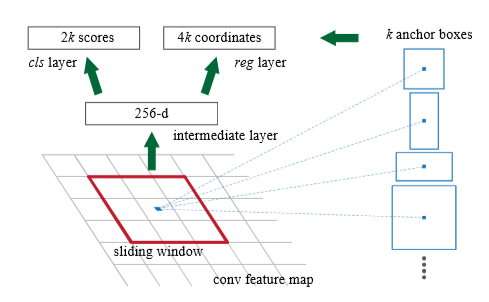
\includegraphics[width=\linewidth]{figure/rpn.png}
        \caption{Region Proposal Network}
    \end{figure}

    \section{You only look once: Unified, real-time object detection\cite{redmon2016you}}

    YOLO网络的基本想法:

    系统将输入图片分为$S\ast S$的网格单元。如果物体的中心落入某个格子,那么这个格子将会用来检测这个物体。每个网格单元会预测B个bounding box以及这些框的置信值。每个bounding box会有5个预测值:x,y,w,h和置信值confidence

    \begin{equation}
        confidence=Pr(Object)\ast IOU^{truth}_{pred}
    \end{equation}

    如果object落在一个网格单元里,$Pr(Object)$取1,否则取0。检测评价函数 intersection-over-union:

    \begin{equation}
        IOU=\frac{DetectionResult\cap GroundTruth}{DetectionResult\cup GroundTruth}
    \end{equation}

    每个网格单元也预测C个条件类概率,$Pr(Class_i|Object)$,在一个网格单元包含一个物体的前提下,它属于某个类的概率。我们只为每个网格单元预测一组类概率,而不考虑框B的数量。在测试的时候,通过如下公式来给出对某一个box来说某一类的confidence score: 
    
    \begin{equation}
        Pr(Class_i|Object)\ast Pr(Object)\ast IOU^{truth}_{pred}=Pr(Class_i)\ast IOU^{truth}_{pred}
    \end{equation}

    然后设定阀值,过滤掉得分低的,对保留的boxes进行NMS处理,得到最终的检测结果。

    网络存在的问题:

    1. 由于输出层为全连接层,只能检测与训练图像相同分辨率的图像。

    2. 虽然每个格子可以预测 B 个 bounding box,但是最终只选择只选择 IOU 最高的 bounding box 作为物体检测输出,即每个格子最多只预测出一个物体。当物体占画面比例较小,如图像中包含畜群或鸟群时,每个格子包含多个物体,但却只能检测出其中一个。

    3. 对于bounding box的误差采用平方误差,没有衡量bounding box的大小。
    
    \section{Ssd: Single shot multibox detector\cite{liu2016ssd}}

    SSD改进了YOLO中一个网格只能预测一个物体的缺点,同时改进网络结构,引入多尺度训练,在保证模型速度的同时提高了模型的准确度。如Figure 5所示,相比YOLO,SSD加入了更多的卷积层,并使用多个不同层次的卷积层做预测,同时用卷积层代替了中间的全连接层,提升了网络的速度。对于不同层的特征图,SSD设置的box会有不同,靠前的特征图用于检测小物体,靠后的特征图用于检测大物体,一定程度上解决了多尺度目标检测的问题。

    \begin{figure}[htb]
        \centering
        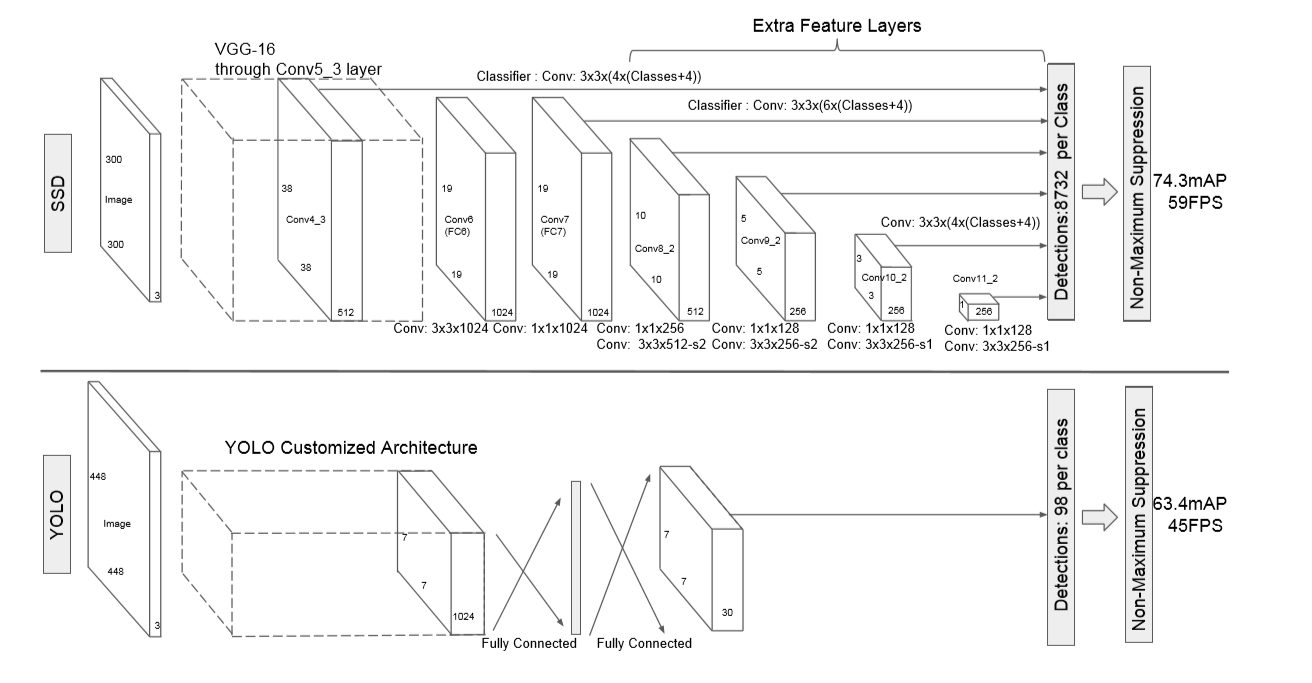
\includegraphics[width=\linewidth]{figure/ssd.png}
        \caption{A comparison between two single shot detection models: SSD and YOLO}
    \end{figure}

    对于正负样本差异的问题,SSD通过confidence loss选择样本,使得正负样本比例最低为1:3。其他的trick包括数据增强、引入更大COCO数据集,增大输入图片大小等。


    \section{图表对比}

    \begin{table}[H]
    \begin{tabular}{|c|c|c|}
        \hline
        Architecture & Performance(VOC 2007) & Speed            \\ \hline
        R-CNN        & 59.2mAP               & $\sim$15s/image  \\ \hline
        SPP Net      & 60.9mAP               & $\sim$0.4s/image \\ \hline
        Fast R-CNN   & 70.0mAP               & $\sim$0.3s/image \\ \hline
        Faster R-CNN & 73.2mAP               & 7FPS             \\ \hline
        YOLO         & 63.4mAP               & 45FPS            \\ \hline
        SSD          & 74.3mAP               & 58FPS            \\ \hline
    \end{tabular}
    \end{table}


    {\small
    \bibliographystyle{IEEEtran} 
    \bibliography{report.bib}
    }

\end{document}